%
% File eamt18.tex
%

\documentclass[11pt]{article}
\usepackage{cs501R}
\usepackage{times}
\usepackage{url}
\usepackage{circuitikz}
\usepackage{latexsym}
\usepackage[framemethod=tikz]{mdframed}
\usepackage[small,bf]{caption} % added MLF 20171211
\setlength\titlebox{6.5cm}    % Expanding the titlebox
%%% YOUR PACKAGES BELOW THIS LINE %%%

%% MJM

\title{XNOR using NAND gate}

\author{ManasaReddy\\
  {\tt manasatanuboddi@gmail.com}}

\date{}

\begin{document}
\maketitle
\section{Contents}
1. Components\\
2. Hardware\\
3. Software\\
\section {Abstract}
This document shows XNOR operation using NAND gates

\section{Components}
\begin{table}[htbp]
 \begin{center}
    \begin{tabular}{|l|c|c|c|c|c|c|} \hline 
  \textbf{Component} & \textbf{Value} & \textbf{Quantity} \\
 \hline
Resistor & 220 Ohm & 1 \\ \hline
Led & - & 1\\ \hline
Arduino & UNO & 1 \\ \hline
Bread board & - & 1 \\ \hline
jumper wires& M-M& 3 \\ \hline
\end{tabular}   
\end{center}
\caption{\label{table:dummytable} Table 1.0}
\end{table}



\section{Hardware}
Make the connections as for Table 1.1
\begin{table}[htbp]
 \begin{center}
    \begin{tabular}{|l|c|c|c|c|c|c|} \hline 
 \textbf{Arduino} & \textbf{13} & \textbf{GND} \\ \hline
 \textbf{Led} & \textbf{+VE} & \textbf{-VE}\\ \hline
\end{tabular}   
\end{center}
\caption{\label{table:dummytable} Table 1.1}
\end{table}


\subsection{XNOR Gate Truth Table}
The truth table of the XNOR gate is shown below:


\begin{figure}[h]
\centering
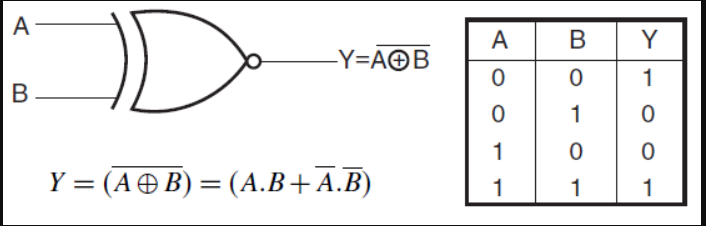
\includegraphics[width=0.4\textwidth]{Capture.PNG}
\caption{\label{capture:XNOR GATE}}
\end{figure}

\begin{circuitikz} \draw
(-1,1) node[nand port] (mynand1) {}
(mynand1.in 1) -- ++ (0,0) node[circ]{} node[left]{$A$}
(mynand1.in 2) -- ++ (0,0) node[circ]{} node[left]{$B$}
(1,2) node[nand port] (mynand2) {}
(mynand1.out) node(X1) [anchor=north]{$X1$}
(1,0) node[nand port] (mynand3) {}
(mynand2.out) node(X2) [anchor=south]{$X2$}
(3,1) node[nand port] (mynand4) {}
(mynand3.out) node(X3) [anchor=north]{$X3$}
(5,1) node [nand port] (mynand5) {}
(mynand4.out) node(X4) [anchor=south]{$X4$}
(mynand5.out) -- ++ (1,0) node[circ]{} node[right]{$Y$}
(mynand2.out) -- (mynand4.in 1)
(mynand3.out) -- (mynand4.in 2)
(mynand1.out) -| (mynand2.in 2)
(mynand1.out) -| (mynand3.in 1)
(mynand4.out) -| (mynand5.in 1)
(mynand4.out) -|(mynand5.in 2)
(mynand1.in 1) |-(mynand2.in 1)
(mynand1.in 2) |-(mynand3.in 2)
;
\end{circuitikz}

EXPRESSIONS FOR XNOR USING NAND\\
GATE\\
X1=(A.B)'\\
X2=(A(A.B)')'\\
X3=((A.B')')\\
X4=(A.B')+(A'.B)\\
Y=((A.B')+(A'.B))'


\section{SOFTWARE}
PROBLEM1:XNOR USING NAND GATE\\
Now make the connections as the table 1.1
Execute the f0llowing program after downloading \\
%\framebox{\\https://github.com/manasareddy442002/fwc-moudle1/blob/main/code.tx
\begin{mdframed}
     https://github.com/manasareddy442002/fwc-moudle1/blob/main/code.txt\
\end{mdframed}
The LED will ON and oFF according to changing XNOR operation
      

\end{document}

